\documentclass[twocolumn, a4j]{article}
\usepackage{multirow}
\usepackage{amsmath,amssymb}
% \usepackage{tgtermes}
\usepackage[T1]{fontenc}
% \usepackage[utf8]{inputenc}
\usepackage[dvipdfmx]{graphicx}
% \usepackage{dblfnote}

\title{「商取引ゲーム」における不正防止の不可能性の証明}
\renewcommand{\thefootnote}{\fnsymbol{footnote}}
\author{Nozomu Miyamoto\footnotemark[2] t16840nm@sfc.keio.ac.jp}
\renewcommand{\thefootnote}{\arabic{footnote}}
\date{\today}

\begin{document}

\twocolumn[
\begin{@twocolumnfalse}
  \maketitle
  \vspace{-6mm}
  \begin{abstract}
    インターネットと電子送金の普及により商取引はよりグローバルに行われるようになった.そんな中,商取引における不正行為は,エスクローと呼ばれる仲介者が信頼できるという前提のもとで防止されている.ただ,この前提は,第3者に依存せずに動作の正当性が保証されており,商取引の当事者の行動を観察できなくとも不正行為防止のためのインセンティブ設計を行えるシステムが存在するという仮定の上で成り立っている.そこで本研究では,そのようなシステムが存在しえるのかを論じるために,先の条件を満たす「商取引システム」とそれを仲介として行う「商取引ゲーム」を定義し,不正行為防止のインセンティブ設計が可能であるかを確認する.その結果として,「商取引ゲーム」において,不正行為防止のインセンティブ設計が不可能であることを証明した.これは本稿で定義される理論上の商取引に基づく限り,商取引において不正行為が行われない合理的な根拠は無いことを意味している.

  \end{abstract}
  \vspace{2mm}
\end{@twocolumnfalse}
]

\renewcommand{\thefootnote}{\fnsymbol{footnote}}
\footnotetext[2]{慶應義塾環境情報学部 NECO Lab.}
\renewcommand{\thefootnote}{\arabic{footnote}}

\section{はじめに}

   インターネットと電子送金の普及によって,国境を超えたグローバルな商取引が瞬時に行えるようになり,我々は日々の生活の中でそれを当然のように受け入れている.また,同時に我々は,国内での電子商取引がそうであったように,このグローバルな商取引でもエスクローサービスと呼ばれる,代金を一時的に預かり商品到着を確認後に支払いを行うサービスを用いることで,詐欺などの不正行為を防止できると信じている.しかしながら,実際のところ,これはエスクローサービスのような商取引の仲介者と別の商取引を結んでいいるに過ぎず,仲介者が信頼できるという前提のもとで成り立っている.\\
   仲介者が信頼できるという前提は,次節で述べる,「第3者に依存しない仲介システム」が存在しているという仮定の上で成り立つものである.また,3節で述べるが,この仮定は,システムから商取引において不正行為を行った当事者が$seller$か$buyer$のどちらであるかを観察できないことを意味している.それ故に,第3者に依存せずに契約での不正行為を防止するシステムは,当事者のうちどちらが不正行為を行ったかという情報を用いずに,当事者達が不正行為を行わないインセンティブ設計を行わなければならない.\\
   本研究の目的は,実社会の商取引において,どのようにして不正行為が抑制されているのかのメカニズムを解明することである.エスクローサービスが電子商取引においては機能しないという前提の上で,電子商取引における不正行為の防止のメカニズムを提案する研究\cite{Shigeo 2000}は存在するものの,暗黙的に商取引の仲介者への信頼が前提となっており,本質的な解決には至っていない.\\
   本稿では,先の条件を満たすシステムを「商取引システム」と呼び,このシステムから参加者達($players$)の通貨の保有量を観察,操作することで商取引のインセンティブ設計を行うものとする.そして,この「商取引システム」を仲介とする商取引を,ゲーム理論を用いて「商取引ゲーム」として定義する.その上で,この「商取引ゲーム」の当事者である$seller$と$buyer$が不正行為を行わないようなインセンティブ設計がシステムから不可能であることを証明し,「商取引ゲーム」において不正行為防止が不可能であることを示す.最後に,今後の研究のため,この理論上の商取引と実社会の商取引を比較することで,なぜ実社会の商取引では不正行為が抑制されているのかを考察する.\\

\section{「第3者に依存しない仲介システム」の必要性}
   商取引において不正行為を防止するためには,第3者に依存せずに動作の正当性が保証された商取引を仲介するシステムが存在していて,かつ,そのシステムは商取引で不正行為を防止できるインセンティブ設計を行える必要がある.仮に第3者に依存せずに動作の正当性が保証された仲介するシステムが存在しないとすれば,再帰的に,商取引を仲介するシステムの動作の正当性を保証する他の仲介するシステムが必要となるため,一向にそのシステムの正当性は保証されない.それ故,必ず第3者に依存せずに動作の正当性が保証された仲介するシステムが存在している必要がある.その上で,商取引において不正行為を防止するには,そのシステムから商取引の当事者達が不正行為を行わなくなるようなインセンティブ設計を行う必要がある.つまりは,第3者に依存せずに動作の正当性が保証されたシステム(本稿では,これを「第3者に依存しない仲介システム」と呼ぶ.)が存在しており,この「第3者に依存しない仲介システム」から商取引の不正行為防止のためのインセンティブ設計が行えなければならない.

  % 仲介者が信頼できるという前提は,第3者に依存せずに契約での不正行為を防止するシステムが存在しているという仮定の上で成り立つ.商取引を行う当事者達($seller$と$buyer$)とその商取引を保証する仲介者が存在するとき,この商取引は$seller$,$buyer$の商取引とその商取引を保証するための$seller$と仲介者の商取引,同じく$buyer$と仲介者の商取引の独立した3つの商取引に分けられる.ここで仲介者が信頼できるという前提が成り立つためには,仲介者との商取引において不正行為が防止されていることが保証されていなければならない.仮に,その商取引を保証するために新たな第3者を仲介者として商取引を結んだとしても,これは新たな第3者を仲介者とする行為が再帰的に繰り返されて,商取引の保証がたらい回しにされているだけである.これを防ぐためには,必ずどこかで,第3者を仲介者とすることなく商取引において不正行為が起きないことを保証するシステムが仲介する必要がある.

  % 商取引において不正行為を防止するためには,第3者に依存せずに動作の正当性が保証されている仲介システムが存在していて,かつ,そのシステムは商取引で不正行為を防止できるインセンティブ設計を行える必要がある.

  % 例えば,アフリカの$seller$と日本の$buyer$が商取引を行うとして,中国のエスクロー業者がその商取引の仲介をするとしよう.ここで日本の$buyer$が代金の入支払いを行ったにも限らず,アフリカの$seller$が商品を発送しなかったとする.当然,日本の$buyer$は中国の仲介者に代金の払い戻しを要求するだろう.しかしながら,ここで中国のエスクロー業者が日本の$buyer$に払い戻しを行うことに,何か合理的な根拠があるだろうか.仮に払い戻しを拒否することが中国の法に違反していたとして,日本の$buyer$のために中国の法が執行されることに何か合理的な根拠があるだろうか.仮に中国の法が執行されることが,国際的か条約で認められていたとして,その約束が守られる合理的な根拠があるだろうか.これは,どこかで他の当事者意外の誰かが約束を守らせようとしなくても,商取引を成立させる仕組みが無い限り,再帰的に仲介者が必要となり,信頼をたらい回しにしているだけである.つまりは,仲介者が信頼できるという前提は,第3者に依存せずに不正行為を防止するシステムが存在しているという仮定の上で成り立つのである.

\section{「行動観察不可の条件」}
  %  第3者に依存せずに不正行為を防止するシステムが存在するとき,そのシステムからは,$seller$と$buyer$が不正を行ったかを観察することはできない.例えば,$seller$と$buyer$の行動を観察するための代理人とシステムが商取引(ここでは,行動を観察して報告することが商品にあたる)を結ばなくてはならず,その時点で,第3者に依存してしまうためである.また,センサーなどを用いて$seller$と$buyer$の行動を観察するにしても,そのセンサーの正当性を保証するために,その製造者などに依存してしまう.つまり,仲介者からは$seller$と$buyer$の行動を観察できない状態で,不正行為を抑制しなければならないのである.
   仮にこのようなシステムが存在していたとして,このシステムからインセンティブ設計を行う際には,商取引の当事者である$seller$と$buyer$の行動を観察することができないという条件(以後,「行動観察不可の条件」と呼ぶ.)をおくべきである.なぜなら,商取引が失敗した場合に$seller$と$buyer$のどちらに非があるかを確かめるには,第3者に依存せずに動作の正当性が保証されているという前提に反して,誰かしらの第3者に依存する必要があるからである.

  例えば,りんごの売買契約を結んだ$seller$と$buyer$がいて,どちらかがシステムにその商取引の失敗を報告したとする.ここで$seller$と$buyer$のどちらが不正行為を行ったかを知るために,代理人を選出して調査を行うことや,りんごにシステムから不正行為を検知するためのセンサーをあらかじめ埋め込むなどの方法がある.しかし,どちらも代理人やセンサーの正当性を保証する製造者などの第3者に依存してしまう.また,代理人や製造者が正当性が保証されたシステムの一部であると仮定しても,第3者である彼らの正当性が保証されているためには,別の「第3者に依存しない仲介システム」を用いて彼らと商取引を結んでいなければならず,その仮定は別の「第3者に依存しない仲介システム」という第3者に依存していることを前提としてしまう.

  つまり,商取引において不正行為を防止するためには,「行動観察不可の条件」を満たす「第3者に依存しない仲介システム」が存在していなければならないのである.

\section{「商取引システム」}
 この「行動観察不可の条件」を満たす「第3者に依存しない仲介システム」が存在するのかを論じるために,このシステムに以下の条件を付随したものを「商取引システム」と定義する.
\begin{itemize}
  \item このシステム内には通貨が存在している.
  \item このシステムからは各$player$(システムの参加者)の通貨の保有量を観察・操作することができる.
  \item このシステムを仲介として商取引を行う際,支払いはシステム内の通貨で行われる.
  \item このシステムは商取引の当事者(本稿では$buyer$)から結果の報告を受けた際に各$player$の通貨の保有量を任意に操作する.
\end{itemize}

\section{「商取引ゲーム」}
 また,この「商取引システム」において,商取引で不正行為を防止できるインセンティブ設計を行うことができるのかを検証するするために,このシステムを商取引の仲介として用いる「商取引ゲーム」を次のように定義する.なお,ここでのゲームの$players$(システムの参加者達)は合理的に(期待利得の最も高い)戦略を決定するものとする.

\subsection{ゲームの進め方}
 本稿での商取引は,以下の4つのステップで$seller$と$buyer$が交互に行動を展開するものとする.

\begin{description}
  \item[step1] $seller$は商品$goods$とその価格を告知する
  \item[step2]  その商品の購入を希望する$buyer$が「商取引システム」に商取引の合意を報告する.
  \item[step3]  $seller$は「正当な行為」と「不正な行為」のどちらかの行動選択をする.ここで「正当な行為」を行った場合,$buyer$は契約通りの$goods$を受け取れ, 「不正な行為」を行った場合,$buyer$は契約通りの$goods$を受け取れないものとする.
  \item[step4]  $buyer$は商取引の「成功」か「失敗」かを「商取引システム」に報告する.この報告に基づき,「商取引システム」は$ seller$と$ buyer$の保有する通貨の量を調整する.
\end{description}

% \textbf{step1} $seller$は商品$goods$とその価格を告知する.
%
% \textbf{step2} その商品の購入を希望する$buyer$が「商取引システム」に商取引の合意を報告する.
%
% \textbf{step3} $seller$は「正当な行為」と「不正な行為」のどちらかの行動選択をする.ここで「正当な行為」を行った場合,$buyer$は契約通りの$goods$を受け取れ, 「不正な行為」を行った場合,$buyer$は契約通りの$goods$を受け取れないものとする.
%
% \textbf{step4} $buyer$は商取引の「成功」か「失敗」かを「商取引システム」に報告する.この報告に基づき,「商取引システム」は$ seller$と$ buyer$の保有する通貨の量を調整する.

\subsection{ゲーム木}
\begin{figure*}[h]
  \centering
  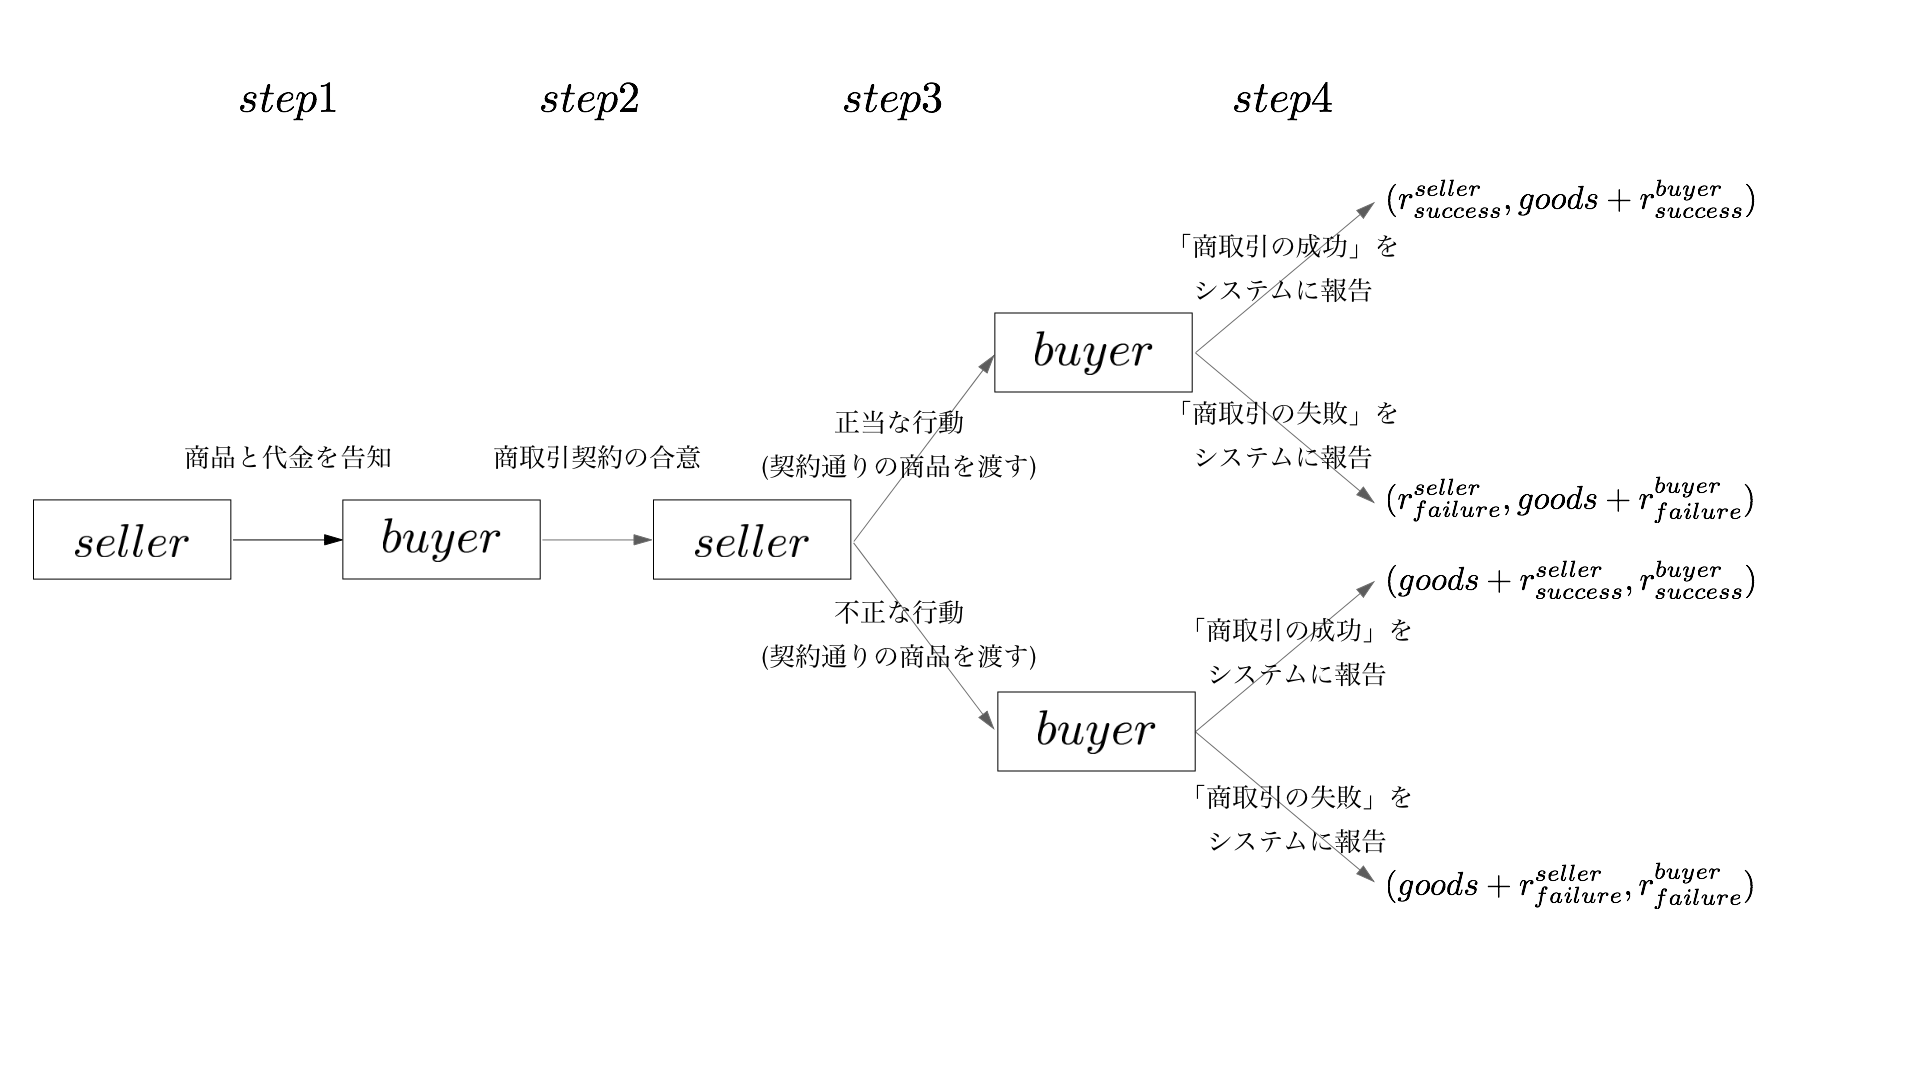
\includegraphics[width=1\linewidth]{gametree.png}
  \caption{「商取引ゲーム」のゲーム木}
  \label{gametree}
\end{figure*}
 先の商取引ゲームをゲームの木を用いて表すと図\ref{gametree}のようになる.\textbf{step1}と\textbf{step2}の時点では商取引の結果が変化することはなく,\textbf{step3}で$seller$が「正当な行為」をとるか否かと,\textbf{step4}での$buyer$からの報告によってのみ商取引の結果は変化する.また,「商取引システム」からは「行動観察不可の条件」より$seller$と$buyer$がどの行動をとったかはわからないため,\textbf{step4}での$buyer$の報告にのみ基づいて$seller$と$buyer$の保有する通貨の量を調整しなければならない.つまりは商取引の結果①と③,②と④はそれぞれ$goods$を除く利得は同じでなくてはならない.


\subsection{非協力戦略型ゲーム}
\newcommand{\successseller}{
  \begin{tabular}{c}
    $(r^{seller}_{success},$\\
    $goods+r^{buyer}_{success})$
  \end{tabular}
}
\newcommand{\successbuyer}{
  \begin{tabular}{c}
    $(goods+r^{seller}_{success},$\\
    $r^{buyer}_{success})$
  \end{tabular}
}
\newcommand{\fseller}{
  \begin{tabular}{c}
    $(r^{seller}_{failure},$\\
    $goods+r^{buyer}_{failure})$
  \end{tabular}
}
\newcommand{\fbuyer}{
  \begin{tabular}{c}
    $(goods+r^{seller}_{failure},$\\
    $r^{buyer}_{failure})$
  \end{tabular}
}

\begin{table*}[h]
\begin{tabular}{|l|l|l|l|l|l|}
\hline
\multicolumn{2}{|l|}{\multirow{2}{*}{}} & \multicolumn{4}{l|}{$buyer$} \\ \cline{3-6}
\multicolumn{2}{|l|}{}                  &$s^{buyer}_1$&$s^{buyer}_2$&$s^{buyer}_3$&$s^{buyer}_4$\\ \hline
\multirow{2}{*}{$seller$}
&$s^{seller}_1$&\successseller&\successseller&\fseller&\fseller\\ \cline{2-6}
&$s^{seller}_2$&\fbuyer&\successbuyer&\fbuyer&\successbuyer\\ \hline
\end{tabular}
\caption{非協力戦略型ゲームとして表した「商取引ゲーム」の利得表}
\label{gametable}
\end{table*}

また,この商取引のモデルは,第3ステップ以降の$seller$の行動選択と,それに対する第4ステップの$ buyer$の行動選択を,非協力戦略型ゲームとしてとらえられる.ここで,戦略$ s^{player}_{n}$を$ player$(ここでは$seller$か$buyer$)の取りうる戦略番号$n$の戦略として,$ seller$と$ buyer$のそれぞれの戦略は以下のように定義する.\\

\begin{description}
  \item[$s^{seller}_1$]… 正当な行為を行う
  \item[$s^{seller}_2$]… 不正な行為を行う
  \item[$s^{buyer}_1$]… $ seller$が正当な行為をとった場合は「成功」を,不正な行動をとった場合は「失敗」を報告する
  \item[$s^{buyer}_2$]… $ seller$が正当な行為をとった場合は「成功」を,不正な行動をとった場合は「失敗」を報告する
  \item[$s^{buyer}_3$]… $ seller$が正当な行為をとった場合は「失敗」を,不正な行動をとった場合は「失敗」を報告する
  \item[$s^{buyer}_4$]… $ seller$が正当な行為をとった場合は「失敗」を,不正な行動をとった場合は「成功」を報告する
\end{description}

% $s^{seller}_1$…「正当な行為を行う」\\
% $s^{seller}_2$…「不正な行為を行う」\\
% $s^{buyer}_1$ …「$ seller$が正当な行為をとった場合は「成功」を,不正な行動をとった場合は「失敗」を報告する」\\
% $s^{buyer}_2$ …「$ seller$が正当な行為をとった場合は「成功」を,不正な行動をとった場合は「成功」を報告する」\\
% $ s^{buyer}_3$ …「$ seller$が正当な行為をとった場合は「失敗」を,不正な行動をとった場合は「失敗」を報告する」\\
% $ s^{buyer}_4$ …「$ seller$が正当な行為をとった場合は「失敗」を,不正な行動をとった場合は「成功」を報告する」\\

また,商取引終了時の$ player$の保有する通貨量の変化によって生じる利得を,第4ステップでの報告が「成功」だった場合は$ r^{player}_{success}$,「失敗」だった場合は$ r^{player}_{failure}$とし,商品の所有によって生じる利得を$ goods$と表す.
ここで,$ seller$と$ buyer$の任意の戦略組$ (s^{seller}_n, s^{buyer}_n)$の際の$ seller$と$ buyer$の各利得は表\ref{gametable}のようになる.

\onecolumn
\section{不可能性の証明}
\subsection{前提の整理}
\begin{itemize}
  \item システムは$buyer$によって報告された商取引の結果を観察できる.
  \vspace{-12mm}
  \item システムは$seller$と$buyer$がどの戦略を選んだかはわからない.
  \vspace{-12mm}
	\item 商取引に参加する$player$は合理的に(利得の期待値が最も高い)戦略を決定する.
  \vspace{-12mm}
	\item システム内には追跡可能な通貨が存在しており,商取引にはその通貨が用いられる.
  \vspace{-12mm}
	\item システムからは$player$の通貨の保有量を操作することができる.
  \vspace{-12mm}
\end{itemize}

\subsection{不正行為が起きない戦略組とその条件}
 表より,商取引で不正行為が起きないためには,$seller$と$buyer$のとる戦略組が$ (s^{seller}_1, s^{buyer}_1)$もしくは$(s^{seller}_1, s^{buyer}_2)$のいずれかに帰着しなければならない.

$(s^{seller}_1, s^{buyer}_1)$に帰着するためには,\\

$E(R|s^{seller}_1)>E(R|s^{seller}_2)$
かつ
$E(R|s^{buyer}_1)>E(R|s^{buyer}_2)$
かつ
$E(R|s^{buyer}_1)>E(R|s^{buyer}_3)$
かつ
$E(R|s^{buyer}_1)>E(R|s^{buyer}_4)$ …条件①\\

を満たす必要があり,$(s^{seller}_1, s^{buyer}_2)$に帰着する場合は,\\

$E(R|s^{seller}_1)>E(R|s^{seller}_2)$
かつ
$E(R|s^{buyer}_2)>E(R|s^{buyer}_1)$
かつ
$E(R|s^{buyer}_2) > E(R|s^{buyer}_3)$
かつ
$E(R|s^{buyer}_2) > E(R|s^{buyer}_4)$ …条件②\\

を満たす必要がある.\\

 つまり,不正行為を防ぐ商取引のインセンティブ設計を行うためには,条件①もしくは条件②を満たす$(r^{seller}_{success}, r^{seller}_{failure}, r^{buyer}_{success}, r^{buyer}_{failure})$の組を「商取引システム」から決定することができなければならない.
そこで,不正行為を防ぐ商取引のインセンティブ設計が不可能であることを示すために,次の命題を証明する.

\subsection{命題}
条件①もしくは条件②のいづれかの条件を満たす$(r^{seller}_{success}, r^{seller}_{failure}, r^{buyer}_{success}, r^{buyer}_{failure})$の組を商取引システムから決定することはできない.

\subsection{証明}
$player$が戦略$s^{player}_n$をとる確率を$p^{player}_{n}$と表す.$(0 \leq p^{player}_{n} \leq 1)$\\

$seller$について,各戦略の期待利得は以下のように表せる. \\
$E(R|s^{seller}_1)=p^{buyer}_1{r}^{seller}_{success}+p^{buyer}_2r^{seller}_{suceess}+p^{buyer}_3r^{seller}_{failure}+p^{buyer}_4r^{seller}_{failure}$ \\

$ E(R |s^{seller}_2) = p^{buyer}_1 (goods + r^{seller}_{failure}) + p^{buyer}_2 (goods + r^{seller}_{success}) + p^{buyer}_3 (goods + r^{seller}_{failure} ) + p^{buyer}_4 (goods + r^{seller}_{success})$ \\

$ = goods + p^{buyer}_1 r^{seller}_{failure} + p^{buyer}_2 r^{seller}_{success} + p^{buyer}_3 r^{seller}_{failure} + p^{buyer}_4 r^{seller}_{success}$ \\

ここで,$E(R |s^{seller}_1) > E(R |s^{seller}_2)$ を満たすためには, \\
$p^{buyer}_1 {r}^{seller}_{success} + p^{buyer}_2 r^{seller}_{suceess} + p^{buyer}_3 r^{seller}_{failure} + p^{buyer}_4 r^{seller}_{failure}$ \\

$ > goods + p^{buyer}_1 r^{seller}_{failure} + p^{buyer}_2 r^{seller}_{success} + p^{buyer}_3 r^{seller}_{failure} + p^{buyer}_4 r^{seller}_{success}$ \\

 $\therefore p^{buyer}_1 {r}^{seller}_{success} +  p^{buyer}_4 r^{seller}_{failure} > goods + p^{buyer}_1 r^{seller}_{failure} + p^{buyer}_4 r^{seller}_{success}$ \\

$\therefore p^{buyer}_1 {r}^{seller}_{success} +  p^{buyer}_4 r^{seller}_{failure} - goods + p^{buyer}_1 r^{seller}_{failure} - p^{buyer}_4 r^{seller}_{success} > 0$ \\

$\therefore p^{buyer}_1(r^{seller}_{success} - r^{seller}_{failure}) - p^{buyer}_4(r^{seller}_{success} - r^{seller}_{failure} ) - goods > 0$ \\

$\therefore (p^{buyer}_1 - p^{buyer}_4)(r^{seller}_{success} - r^{seller}_{failure}) - goods> 0$ \\

$\therefore (p^{buyer}_1 - p^{buyer}_4)(r^{seller}_{success} - r^{seller}_{failure} - \frac{ goods }{p^{buyer}_1 - p^{buyer}_4})> 0$ \\
を満たす必要がある.つまり,\\

$ p^{buyer}_1>p^{buyer}_4$のときは, \\

$ r^{seller}_{success} - r^{seller}_{failure} > \frac{ goods }{p^{buyer}_1 - p^{buyer}_4}$\\

$ p^{buyer}_1 < p^{buyer}_4$のときは,\\

$ r^{seller}_{success} - r^{seller}_{failure} < \frac{ goods }{p^{buyer}_1 - p^{buyer}_4}$\\

を満たせば,$E(R |s^{seller}_1) > E(R |s^{seller}_2)$である.
なお,$ p^{buyer}_1 = p^{buyer}_4$のときは,\\

$E(R |s^{seller}_1) > E(R |s^{seller}_2)$は成り立たない.\\

また,$ {buyer}$について,各戦略の期待利得は以下のように表せる.\\

$ E(R|s^{buyer}_1) = p^{seller}_1 (goods + r^{buyer}_{success}) + p^{seller}_2 r^{buyer}_{failure}$ \\

$ E(R|s^{buyer}_2)=p^{seller}_1 (goods + r^{buyer}_{success}) + p^{seller}_2 r^{buyer}_{success}$ \\

$ E(R|s^{buyer}_3)=p^{seller}_1 (goods + r^{buyer}_{failure}) + p^{seller}_2 r^{buyer}_{failure}$ \\

$ E(R|s^{buyer}_4)=p^{seller}_1 (goods + r^{buyer}_{failure}) + p^{seller}_2 r^{buyer}_{success}$ \\

\subsubsection{条件①が成り立たないことの証明}

ここで,条件①の必要条件である
$E(R|s^{buyer}_1)>E(R|s^{buyer}_2)$
かつ
$E(R|s^{buyer}_1)>E(R|s^{buyer}_3)$
かつ
$E(R|s^{buyer}_1)>E(R|s^{buyer}_4)$
を満たすためには,\\

$ E(R|s^{buyer}_1) > E(R|s^{buyer}_2)$ \\

$\therefore p^{seller}_1 (goods + r^{buyer}_{success}) + p^{seller}_2 r^{buyer}_{failure} > p^{seller}_1 (goods + r^{buyer}_{success}) + p^{seller}_2 r^{buyer}_{success}$ \\

$\therefore p^{seller}_2 r^{buyer}_{failure} - p^{seller}_2 r^{buyer}_{success} > 0$ \\

$\therefore p^{seller}_2 (r^{buyer}_{failure} - r^{buyer}_{success}) > 0$ \\

つまり,$ p^{seller}_2 > 0$ かつ $ r^{buyer}_{failure} - r^{buyer}_{success} > 0$

\begin{equation}
  p^{seller}_2 > 0
\end{equation}

\begin{equation}
\label{quad1}
  0 > r^{buyer}_{success} - r^{buyer}_{failure}
\end{equation}

$ E(R|s^{buyer}_1) > E(R|s^{buyer}_3)$ \\

$ p^{seller}_1(goods + r^{buyer}_{success}) + p^{seller}_2r^{buyer}_{failure}>
  p^{seller}_1(goods + r^{buyer}_{failure}) + p^{seller}_2r^{buyer}_{failure}$\\

$ p^{seller}_1 (r^{bueyer}_{success} - r^{buyer}_{failure}) > 0$\\

つまり,$ p^{seller}_1 > 0$ かつ $r^{bueyer}_{success} - r^{buyer}_{failure} > 0$\\

\begin{equation}
   p^{seller}_1 > 0
\end{equation}
\begin{equation}
   \label{quad2}
   r^{buyer}_{success} - r^{buyer}_{failure} > 0
\end{equation}

$ E(R|s^{buyer}_1) > E(R|s^{buyer}_4)$ \\

$\therefore p^{seller}_1 (goods + r^{buyer}_{success}) + p^{seller}_2 r^{buyer}_{failure} > p^{seller}_1 (goods + r^{buyer}_{failure}) + p^{seller}_2 r^{buyer}_{success}$ \\

$\therefore p^{seller}_1(r^{buyer}_{success} - r^{buyer}_{failure}) + p^{seller}_2(r^{buyer}_{failure} - r^{buyer}_{success}) > 0$ \\

$ (p^{seller}_1 - p^{seller}_2)(r^{buyer}_{success} - r^{buyer}_{failure}) > 0$\\

\begin{equation}
\label{quad3}
  (p^{seller}_1 - p^{seller}_2)(r^{buyer}_{success} - r^{buyer}_{failure}) > 0
\end{equation}

の3つを満たす必要がある.しかし,(\ref{quad1})と(\ref{quad2})は矛盾するため,
$(r^{seller}_{success}, r^{seller}_{failure}, $
$r^{buyer}_{success}, r^{buyer}_{failure})$ \\
がいかなる実数の組でも条件①は成り立たない. \\


\subsubsection{条件②が成り立たないことの証明}
また,条件②の必要条件である
$E(R|s^{seller}_1)>E(R|s^{seller}_2)$
かつ
$E(R|s^{buyer}_2)>E(R|s^{buyer}_1)$
かつ
$E(R|s^{buyer}_2) > E(R|s^{buyer}_3)$
かつ
$E(R|s^{buyer}_2) > E(R|s^{buyer}_4)$
を満たすためには,

$ E(R|s^{buyer}_2) > E(R|s^{buyer}_1)$ \\

$\therefore p^{seller}_1 (goods + r^{buyer}_{success}) + p^{seller}_2 r^{buyer}_{success} > p^{seller}_1 (goods + r^{buyer}_{success}) + p^{seller}_2 r^{buyer}_{failure}$\\

$\therefore p^{seller}_2 (r^{buyer}_{success} - r^{buyer}_{failure}) > 0$\\

$0 \leq p^{seller}_2 \leq 1$より,\\

$p^{seller}_2 > 0$かつ
$r^{buyer}_{success} - r^{buyer}_{failure} > 0$\\

\begin{equation}
  p^{seller}_2 > 0
\end{equation}

\begin{equation}
  \label{quad2-1}
  r^{buyer}_{success} - r^{buyer}_{failure} > 0
\end{equation}

$ E(R|s^{buyer}_2) > E(R|s^{buyer}_3)$\\

$\therefore p^{seller}_1 (goods + r^{buyer}_{success}) + p^{seller}_2 r^{buyer}_{success} > p^{seller}_1 (goods + r^{buyer}_{failure}) + p^{seller}_2 r^{buyer}_{failure}$\\

$\therefore p^{seller}_1 (r^{buyer}_{success} - r^{buyer}_{failure}) + p^{seller}_2 (r^{buyer}_{success} - r^{buyer}_{failure}) > 0$\\

$\therefore (p^{seller}_1 + p^{seller}_2)(r^{buyer}_{success} - r^{buyer}_{failure}) > 0$\\

$ p^{seller}_1 + p^{seller}_2 = 1 > 0$より,\\

$ r^{buyer}_{success} - r^{buyer}_{failure} > 0$\\

\begin{equation}
  \label{quad2-2}
  r^{buyer}_{success} - r^{buyer}_{failure} > 0
\end{equation}

$ E(R|s^{buyer}_2) > E(R|s^{buyer}_4)$\\

$\therefore p^{seller}_1 (goods + r^{buyer}_{success}) + p^{seller}_2 r^{buyer}_{success} > p^{seller}_1 (goods + r^{buyer}_{failure}) + p^{seller}_2 r^{buyer}_{success}$\\

$\therefore p^{seller}_1(r^{buyer}_{success} - r^{buyer}_{failure}) > 0$\\

$ p^{seller}_1 > 0$かつ
$ r^{buyer}_{success} - r^{buyer}_{failure} > 0$\\

\begin{equation}
  p^{seller}_1 > 0
\end{equation}

\begin{equation}
  \label{quad2-3}
  r^{buyer}_{success} - r^{buyer}_{failure} > 0
\end{equation}

ここで,(\ref{quad2-1}),(\ref{quad2-2}),(\ref{quad2-3})を満たす
$ (r^{buyer}_{success}, r^{buyer}_{failure})$の組はシステムから決定できるため,\\

$p^{seller}_2>0$かつ$p^{seller}_1>0$であれば,

$E(R|s^{buyer}_2)>E(R|s^{buyer}_1)$
かつ
$E(R|s^{buyer}_2) > E(R|s^{buyer}_3)$
かつ
$E(R|s^{buyer}_2) > E(R|s^{buyer}_4)$
を満たすことができる.\\

ここで仮に$p^{seller}_2>0$かつ$p^{seller}_1>0$が成り立ち$ buyer$が戦略$ s^{buyer}_2$を選択するととする.\\

このとき,$buyer$が各戦略をとる確率$(p^{buyer}_1, p^{buyer}_2, p^{buyer}_3, p^{buyer}_4)$は$ (0, 1, 0, 0)$と表せる.\\

ここで,$ p^{buyer}_1 = p^{buyer}_4 = 0$のため,
$E(R |s^{seller}_1) > E(R |s^{seller}_2)$は成り立たない.\\

それゆえに,条件②は成り立たない.\\

以上より,条件①もしくは条件②のいづれかの条件を満たす
$(r^{seller}_{success}, r^{seller}_{failure},$
$r^{buyer}_{success},r^{buyer}_{failure})$の組を「商取引システム」から決定することはできない.\\

\twocolumn
\section{結論}
   本稿では,商取引において不正行為を防止するためには,「行動観察不可の条件」を満たした「第3者に依存しない仲介システム」が存在している必要があることを論じた.その上で,そのシステムが存在するのかを検証するために,下記の条件を付随した「商取引システム」と,それを仲介とした「商取引ゲーム」を定義して,商取引で不正行為を防止できるインセンティブ設計が可能かを確かめた.

  \begin{itemize}
    \item システムは$buyer$によって報告された商取引の結果を観察できる.
    \item システムは$seller$と$buyer$がどの戦略を選んだかはわからない.
    \item 商取引に参加する$player$は合理的に(利得の期待値が最も高い)戦略を決定する.
    \item システム内には追跡可能な通貨が存在しており,商取引にはその通貨が用いられる.
    \item システムからは$player$の通貨の保有量を操作することができる.
  \end{itemize}

  その結果として,不正行為が防止されるための2つの戦略組のいずれかに$seller$と$buyer$の戦略を帰着させるような利得の組を商取引システムから決定することはできないことを証明した.これはつまり,人々は合理的であるという仮定の上で成り立つ「商取引ゲーム」において,不正行為を防止することが不可能であることを意味する.


\section*{考察}
 本稿で論じた理論上の商取引(「商取引ゲーム」)において不正行為防止は不可能であるという結論に反して,我々が日々を暮らす実社会では商取引での不正行為はある程度,抑制されている.この原因は,理論上の商取引の前提と実社会の商取引の差異にあるはずである.1つ考えられるのは,$buyer$側の戦略に含まれる「$seller$が不正行為を行った場合に「成功」を報告する」という行動だ.理論上の商取引においては,この行動を含む戦略は他の戦略に比べて期待利得が高く合理的な戦略であるといえるが,実社会ではこの行動が取られることは稀である.メルカリやヤフオクなどの商取引プラットフォームでは,多くのユーザーが商取引で相手が不正行為を行ったとき,相手からの報復で「悪い評価」をつけられることを恐れずに,相手に「悪い評価」をつけている.また,同様に多くのユーザーが不正行為を働いた場合に相手が「悪い評価」をつけてくると考えているために,誠実な行動をとっている.つまりは,$seller$が不正行為を行った場合に必ず「失敗」を報告しているという仮定が置かれていると考えられる.今後の研究では,この仮定をおいた上で,「商取引システム」から「商取引ゲーム」で不正行為が防止されるようなインセンティブ設計が可能であるかどうかを明らかにするとともに,それが可能であるならば,その仮定を守る$player$の割合が,不正行為の発生率にどのように影響をもたらすかを検証したい.

% 我々がヤフオクやメルカリなどの商取引プラットフォーム上で,商取引を行う際,仮に不正行為にあったとしても,その商取引プラットフォームとの契約に基づいて彼らが負債を負担してくれており,その契約が反故にされることは稀である.仮に彼らが契約を反故にしたとしても,そのさらなる仲介者である法を司る裁判所が,裁判所が反故にしたなら国家が,国家がそれに応じなければ国家の信用を担保するものが不正を正してくれると我々は信じられている.しかし,本研究の理論上は,ここには不正行為が防止される根拠は何も存在しない.では,なぜ実社会では不正行為がある程度抑制されているのだろうか.
%
% この原因は$ buyer$側の戦略に含まれる「$seller$が不正行為を行った場合に「成功」を報告する」という行動が実社会ではほとんど取られていないためではないかと考えられる.我々は先に挙げたようなプラットフォームで不正行為にあった場合,多くがプラットフォームに対して商取引の「失敗」を報告する.つまりは,本稿の理論によれば不合理な行動をとるわけである.
% すべての$player$が「$seller$が不正行為を行った場合に「失敗」を報告する」と仮定すれば,$buyer$の戦略は$s^{buyer}_1$と$s^{buyer}_3$のいずれかになり,

\section*{謝辞}
 所属する研究会である慶應SFC村井研NECO Lab.の指導教員の斉藤賢爾氏と入会時よりお世話になっている阿部涼介氏,及び,今学期のKGLをなさっていた菅藤佑太氏,そのほかNECO lab.の方々への感謝をここに記します.

\renewcommand{\refname}{参考文献}
\begin{thebibliography}{数字}
  \bibitem[Shigeo 2000]{Shigeo 2000} Shigeo Mastubara and Makoto Yoko, Fraud-Free Exchange Mechanisms in Electronic Commerce, Journal of Japanese Society for Artificial Intelligence(2000).
\end{thebibliography}

\end{document}
